\scanpage{10}
\uline{Exercise} \handwritten{4}.\handwritten{10}.\handwritten{6} . Let \(S\) be a \(\underline{U}\)-site whose topology is coarser than the canonical one , \(\underline{\deleted{\unsure{S}}\handwritten{M}}\) a subset of \(\mathrm{Fl}(S)\) having the following properties :

 a) The morphisms of \(\underline{M}\) are base-changeable (I \handwritten{10}.\handwritten{3}) and \(\underline{\unsure{\deleted{S}M|\deleted{M}S}}\) is stable under base change.

% The overtyping-order doubt marked in a) also applies to the repeated form in b).
 b) \(\underline{\deleted{S}M}\) contains the identity arrows and is stable under composition .

 c) An arrow \(u:X\to Y\) such that there exists a covering family \(Y_i\to Y\) , with the \(X\times_Y Y_i\to Y_i\) in \(\underline{M}\) , is itself in \(\underline{M}\) .

 d) For every object \(X\) , every covering family of \(X\) is refined by a covering family \((f_i:X_i\to X)\) where the \(f_i\) are in \(\underline{M}\).

For every object \(X\) , \deleted{let us consider the site}\inserted{let us denote by} \(S(X)\) (``small site of \(X\)'')%
% Matching handwritten looped insertion signs: attachment in the text and words in the left margin.
\handwritten{
\begin{tikzpicture}[x=1pt,y=1pt,baseline=-1pt]
\draw[line width=.55pt,line cap=round] (0,0) .. controls (1.7,4.8) and (4.2,8.8) .. (5.5,11.3);
\draw[line width=.55pt,line cap=round] (5.5,11.3) .. controls (3.6,10.7) and (3.9,14.2) .. (5.7,14.4) .. controls (8.6,14.4) and (8.6,11.2) .. (5.5,11.3);
\end{tikzpicture}}%
\reversemarginpar
\margin{\handwritten{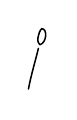
\begin{tikzpicture}[x=1pt,y=1pt,baseline=-2pt]
\draw[line width=.55pt,line cap=round] (0,-1) .. controls (1,4.3) and (2.5,9.1) .. (3.6,13.7);
\draw[line width=.55pt,line cap=round] (4.1,15) .. controls (2.8,15.8) and (3.5,19.6) .. (4.8,20.8) .. controls (7,20.9) and (6.6,15.6) .. (4.1,15);
\end{tikzpicture}}\inserted{the site}}
\normalmarginpar
\deleted{whose underlying category is}\inserted{consisting of} the full subcategory of \(S/X\) formed of the objects whose structure morphism is in \(\underline{M}\) , equipped with the topology induced by that of \(S\) (III \handwritten{3}.\handwritten{1}).

1) Show that the covering families \((f_i:X_i\to X)_{i\varepsilon I}\) where the \(f_i\) are in \(\underline{M}\) form a pretopology on \(S\) (II \handwritten{1}.\handwritten{3}) which generates the topology of \(S\) .

2) For every arrow \(u:X\to Y\) of \(S\) , show that the functor of base change by \(u\) is a continuous functor (III \handwritten{1}.\handwritten{1}) from \(S(Y)\) to \(S(X)\) . \unsure{\(\mathbb{O}\)|\deleted{o}O|\deleted{O}o}ne will denote by
\[
S(u)^{\handwritten{*}}:S(Y)^{\handwritten{\sim}}\to S(X)^{\handwritten{\sim}}
\]
the corresponding functor between the categorie\handwritten{s} of sheaves (III \handwritten{1}.\handwritten{2},iv)).

3) Define an equivalence between the topos \(S^{\handwritten{\sim}}\) and the category of systems
\[
(F_X)\ (X\varepsilon\operatorname{ob}S)\quad,\quad(\handwritten{\varphi_u})\ (u\varepsilon\mathrm{Fl}\ S)
\]
consisting of objects \(F_X\varepsilon\operatorname{ob}S(X)^{\handwritten{\sim}}\) , and for every arrow \(u:X\to Y\) in \(S\) , of a morphism \(\handwritten{\varphi}_u:S(u)^{\handwritten{*}}(F_Y)\to F_X\) , these systems
% archive sheet number: 9
